% !TEX root = Entwurf_goApp.tex

\section{Client} 
	\hypertarget{controler.service}{}
	\subsection{edu.kit.pse.gruppe1.goApp.client.controler.service}
	Im folgenden Kapitel werden alle Services die von unserer App implementiert werden beschrieben.
	Sie alle erben von der Klasse IntentService, weshalb wir zusätzlich zum Konstruktor nur eine public Methode für jeden Service implementieren und zwar die Methode onHandleIntent(Intent intent).
	Weil diese Methode bei all unseren Services nur je nach Intent entscheidet, welche private Methode aufgerufen wird und das Ergebnis weiterleitet, haben wir uns dazu entschieden im folgenden nicht für jeden Service auf die besagte Methode einzugehen sondern jeweils die Methoden zu beschreiben welche durch onHandleIntent(Intent intent) aufgerufen werden, da dies unserer Meinung nach eine bessere Definition der Services Klassen liefert und damit für bessere Verständlichkeit sorgt. 
	
	\subsubsection {LoginService extends IntentService}
		This Service takes care of the identification process of a User and is needed whenever an User starts the App.
	\newline Methods:
	\begin{itemize}
	\item private User login(Int userID)
		\begin{description}
		\item Checks if the user is already registered and gets the users data from the server database.
	 	\item @param UserID the id of the user which has to be found in the server database.
	 	\item @return The user who is now logged in.
		\end{description}
	\end{itemize}
	
	\subsubsection {UserService extends IntentService}
		This Service provides methods to handle a single user.
	\newline Methods:
	\begin{itemize}
	\item private boolean changeName(User user, String name)
		\begin{description}
		\item Changes the old name into the new name of a user.
	 	\item @param user The user who changes his name
	 	\item @param name The new name
	 	\item @return true, if method was successful, otherwise false
		\end{description}
	\end{itemize}
	
	\subsubsection {GroupService extends IntentService}
		This Service provides methods to handle a single group.
	\newline Methods:
	\begin{itemize}
	\item private boolean create(String name, User founder)
		\begin{description}
		\item Creates a new Group.
	 	\item @param name The name of the new group.
	 	\item @param founder The user who creates the group.
	 	\item @return true, if method was successful, otherwise false
		\end{description}
	\item private boolean delete(Group group) 
		\begin{description}
		\item Deletes a group.
	 	\item @param group The group to be deleted.
	 	\item @return true, if methode was successful, otherwise false
		\end{description}
	\item private boolean deleteMember(Group group, User user) 
		\begin{description}
		\item Removes a member from the group.
	 	\item @param group The group in which the user currently is but will be deleted from.
	 	\item @param user The user who will be removed from the group.
	 	\item @return true, if method was successful, otherwise false.
		\end{description}
	\item private boolean setName(Group group, String newName) 
		\begin{description}
		\item Changes the name of the group.
	 	\item @param group The group which's name will be changed.
	 	\item @param newName The new name of the group.
	 	\item @return true, if method was successful, otherwise false.
		\end{description}	
	\item private Group getGroup(int groupID)
		\begin{description}
		\item Gets the group from the server database.
	 	\item @param groupID The unique id of the group.
	 	\item @return The group with the given id or null if it doesn't exist.
		\end{description}	
	\item private boolean setFounder(Group group, User newFounder)
		\begin{description}
		\item Changes the founder of the group.
	 	\item @param group The group which founder changes.
	 	\item @param newFounder The user who gets the rights of the founder.
	 	\item @return true, if method was successful, otherwise false.
		\end{description}	
	\item private List<Event> getEvents(Group group)
		\begin{description}
		\item Returns all events which are associated with the group or null if no events exist in this group.
	 	\item @param group The existing group to get events from.
	 	\item @return all events in the group or null.
		\end{description}	
	\end{itemize}
	
	\subsubsection {GroupSearchService extends IntentService}
		This Service is needed to list various groups at once.
	\newline Methods:
	\begin{itemize}
	\item private List<Group> getGroupsByMember(User user)
		\begin{description}
		\item Finds all groups which the user is a member of. This is used to present the groups in the StartActivity.
	 	\item @param user The user whose groups are returned.
	 	\item @return All groups the user is member of or null.
		\end{description}
	\item private List<Group> getGroupsByName(String name)
		\begin{description}
		\item Finds all groups which name include the given String to show the results of a search request by the user using the search function of the NewGroupActivity.
	 	\item @param name The String which the user typed in the NewGroupActivity to find a new group he wants to be member of.
	 	\item @return All groups where the name is included in the group name or null.
		\end{description}
	\end{itemize}
	
	\subsubsection {RequestService extends IntentService}
	This Service provides methods to handle a Request.
	\newline Methods:
	\begin{itemize}
	\item private boolean create(User user, Group group)
		\begin{description}
		\item Creates a new Request.
	 	\item @param user The user who sends the request.
	 	\item @param group The group the user wants to be a member of.
	 	\item @return true, if method was successful, otherwise false
		\end{description}
	\item private private boolean accept(Request request)
		\begin{description}
		\item Adds the user to the group and deletes the Request if the founder of the group allows the user to join in the group.
	 	\item @param request The request the founder has made a decision about.
	 	\item @return true, if method was successful, otherwise false
		\end{description}
	\item private boolean reject(Request request)
		\begin{description}
		\item Deletes the request if the founder decides that the user will not join in the group.
	 	\item @param request the request the founder has made a decision about.
	 	\item @return true, if method was successful, otherwise false.
		\end{description}
	\end{itemize}
	
	\subsubsection {RequestSearchService extends IntentService}
	This Service is used to list Requests.
	\newline Methods:
	\begin{itemize}
	\item private List<Group> getRequestsByUser(User user) 
		\begin{description}
		\item Finds all requests of a given user. This is used to show all the requests to this user in the StartActivity.
	 	\item @param user The user who created the requests.
	 	\item @return All groups where the user requested to join or null.
		\end{description}
	\item private List<User> getRequestsByGroup(Group group) 
		\begin{description}
		\item Finds all access requests to a given group. This is used to present the requests to the founder of the group to let him decide about them in the GrouInfoActivity.
	 	\item @param group The existing group which founder wants to access the requests.
	 	\item @return All users who want to join the group or null.
		\end{description}
	\end{itemize}
	
	\subsubsection {ParticipateService extends IntentService}
		This Service provides methods to handle a users reaction towards an event.
	\newline Methods:
	\begin{itemize}
	\item private private boolean accept(Event event, User user)
		\begin{description}
		\item The user is added to the event as a participant this includes starting a timer for the notification broadcast. This method is used if the user wants to participate and enters this decision in the GroupActivity.
	 	\item @param event The event where the user wants to participate in. User and event have to be in the same group.
	 	\item @param user The user who wants to participate and is in the same group as the event.
	 	\item @return true, if method was successful, otherwise false
		\end{description}
	\item private boolean reject(Event event, User user)
		\begin{description}
		\item The connection between the user and the event is deleted.
	 	\item @param event The event which the user doesn't want to join.
	 	\item @param user The user who doesn't want to participate.
	 	\item @return true, if method was successful, otherwise false
		\end{description}
	\end{itemize}
		
	\subsubsection {LocationService extends IntentService }
	This Service is in charge of synchronizing the Users and the Group Location.
	\newline Methods:
	\begin{itemize}
	\item private boolean syncLocation(User user, Event event)
		\begin{description}
		\item Sends the clients current location to the server and updates the group location of the event on the client. This method is started at a specific time and is performed periodically.
	 	\item @param user The user whose location is updated.
	 	\item @param event The event which's group locations are returned.
	 	\item @return true, if method was successful, otherwise false
		\end{description}
	\end{itemize}
	
	\subsubsection {public class EventService extends IntentService}
	This Service provides methods to handle a single event.
	\newline Methods:
	\begin{itemize}
	\item private boolean create(String name, Location destination, User eventAdmin, Time time, Group group)
		\begin{description}
		\item  Creates an event.
		\item @param name The name of the event chosen freely by a member of the group.
	 	\item @param destination The location which the user choose on a map to let his event take place.
	 	\item @param eventAdmin The user who creates the event and is a group member.
	 	\item @param time The time when the event is going to take place. This time can not be in the past.
		\item @param group The group in which the event is created and which members are all invited.
	 	\item @return true, if method was successful, otherwise false
		\end{description}
	\item private Event getEvent(int eventID)
		\begin{description}
		\item Gets the event from the server database.
	 	\item @param eventID The id to identify which event to get.
	 	\item @return An event object with attributes.
		\end{description}
	\item private boolean change(Event event)
		\begin{description}
		\item if the event admin whishes to change the event. Only time, destination and name can be changed.
		\item @param event The new instance of the event with the wanted attributes changed which will replace the old event.
		\item @return true, if method was successful, otherwise false
		\end{description}
	\end{itemize}
	
	\subsubsection {GoService extends IntentService}
		This Service provides methods to handle if the user already left for the destination of the event.
	\newline Methods:
	\begin{itemize}
	\item private boolean setGo(User user, Event event)
		\begin{description}
		\item Adds the user to the list of users who are on their way to the event.
	 	\item @param user The user who starts. This user has to be a member of the group in which the event is and has to be a participant of this event.
	 	\item @param event The event on which the user participates.
	 	\item return true, if method was successful, otherwise false
		\end{description}
	\item private List<User> getStartedParticipants(Event event) 
		\begin{description}
		\item Finds all participants of an event whom have started. This is used by the EventActivity to show which participants are on their way.
	 	\item @param event The event you want to know about.
	 	\item @return Every user who's status indicates started, which means that they are on the way to the event.
		\end{description}
	\end{itemize}
	
	 \subsubsection {NotificationService extends IntentService}
		This Service is used to notify an user that an event has started, even when the Application is closed via the Notificationbar.
	\newline Methods:
	\begin{itemize}
	\item private void notify()
		\begin{description}
		\item Send a notification to the user that the event is going to start.
		\end{description}
	\end{itemize}
	
		\hypertarget{view}{}
	\subsection{edu.kit.pse.gruppe1.goApp.client.view}
	In diesem Abschnitt werden die Activities der goApp und ihre Interaktionen mit den Services sowie die Übergänge zu anderen Activities vorgestellt.
	Da die Activities die GUI des Benutzers bilden, werden hier ebenfalls die GUI-Ausschnitte aus dem Pflichtenheft, mit zusätzlichen Erweiterungen, den entsprechenden Activities durch welche sie dargestellt werden zugeordnet.  
	
	\subsubsection {LoginActivity}
	Die LoginActivity wird mit der App gestartet, hier kann sich ein Benutzer registrieren.
	\newline
	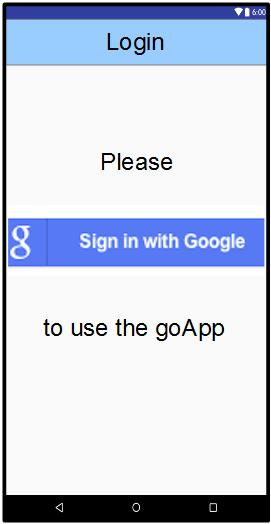
\includegraphics[width=.3\textwidth]{GUI_Login.jpg}
	\newline
	Services die von dieser Activity gestartet werden:
	\begin{itemize}
	\item LoginService
	\end{itemize}
	Von dieser Activity kann ein Benutzer zu folgenden Activities navigieren:
	\begin{itemize} 
	 \item StartActivity
	\end{itemize}
	
	\subsubsection {StartActivity}
	Die StartActivity gibt dem Benutzer eine Übersicht über alle Gruppen in denen er Mitglied ist und denen er eine Beitrittsanfrage geschickt hat.
	Außerdem kann hier der Benutzername geändert werden.
	\newline
	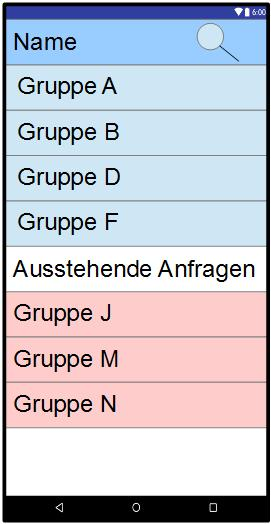
\includegraphics[width=.3\textwidth]{GUI_Start.jpg}
	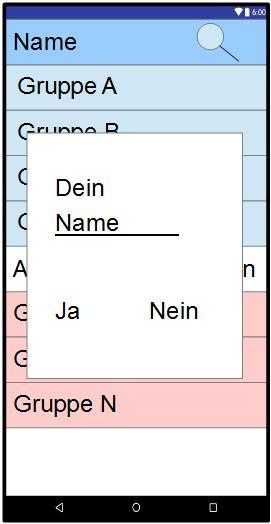
\includegraphics[width=.3\textwidth]{GUI_Start2.jpg}
	\newline
	Services die von dieser Activity gestartet werden:
	\begin{itemize}
	\item UserService
	\item GroupService
	\item GroupSearchService
	\item RequestSearchService
	\end{itemize}
	Von dieser Activity kann ein Benutzer zu folgenden Activities navigieren:
	\begin{itemize} 
	\item GroupActivity
	\item NewGroupActivity
	\end{itemize} 
	
	\subsubsection {GroupActivity}
	Die GroupActivity zeigt dem Benutzer alle anstehenden Termine einer Gruppe, bei denen er nicht abgesagt hat, an.
	\newline
	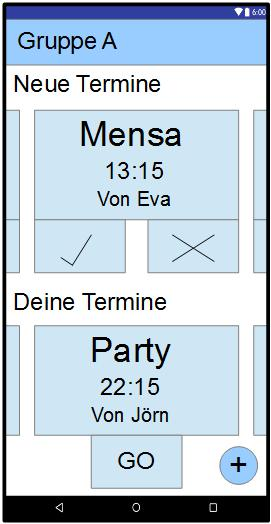
\includegraphics[width=.3\textwidth]{GUI_Group.jpg}
	\newline
	Services die von dieser Activity gestartet werden:
	\begin{itemize}
	\item EventService
	\item ParticipateService
	\item GoService
	\end{itemize}
	Von dieser Activity kann ein Benutzer zu folgenden Activities navigieren:
	\begin{itemize} 
	 \item StartActivity
	 \item GroupInfoActivity
	 \item EventActivity
	 \item NewEventActivity
	\end{itemize} 
	
	\subsubsection {GroupInfoActivity}
	Die GroupInfoActivity zeigt einem Mitglied der Gruppe deren Mitglieder an und bietet die Möglichkeit aus der Gruppe auszutreten. Der Gruppengründer sieht zusätzlich Beitrittsanfragen an die Gruppe und kann diese bearbeiten, er kann auch Mitglieder entfernen und die Gruppe löschen.
	\newline
	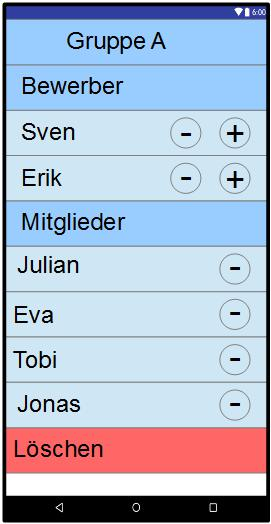
\includegraphics[width=.3\textwidth]{GUI_GruppeInfoGruender.jpg}
	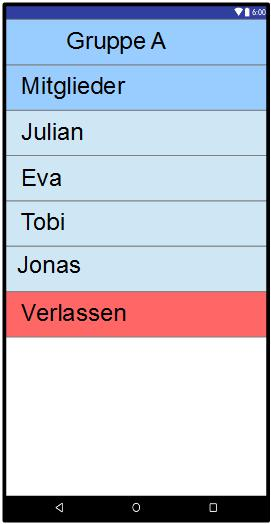
\includegraphics[width=.3\textwidth]{GUI_GruppeInfoNormal.jpg}
	\newline
	Services die von dieser Activity gestartet werden:
	\begin{itemize}
	\item GroupService
	\item RequestService
	\item RequestSearchService
	\end{itemize}
	Von dieser Activity kann ein Benutzer zu folgenden Activities navigieren:
	\begin{itemize} 
	 \item GroupActivity
	 \end{itemize}
	 
	\subsubsection {NewGroupActivity}
	Die NewGroupActivity ermöglicht es einem Benutzer nach Gruppen zu suchen um diesen Beitrittsanfragen zu schicken und neue Gruppen zu erstellen.
	\newline
	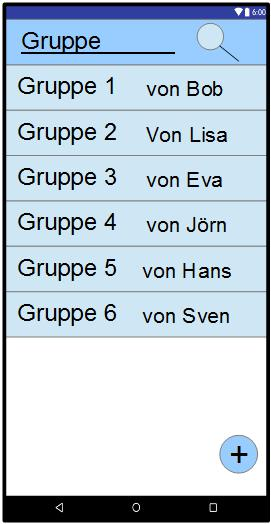
\includegraphics[width=.3\textwidth]{GUI_NeueGruppe.jpg}
	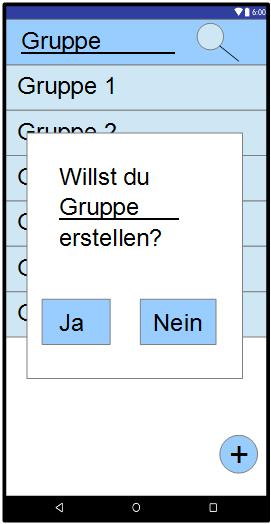
\includegraphics[width=.3\textwidth]{GUI_GruppeNeuBest.jpg}
	\newline
	Services die von dieser Activity gestartet werden:
	\begin{itemize}
	\item GroupService
	\item GroupSearchService
	\item RequestService
	\end{itemize}
	Von dieser Activity kann ein Benutzer zu folgenden Activities navigieren:
	\begin{itemize} 
	 \item StartActivity
	 \item GroupActivity
	 \end{itemize}
	 
	\subsubsection {EventActivity}
	Die EventActivity lässt einen Benutzer alle Informationen zu einem Termin einsehen und bindet eine dynamische Karte ein.
	\newline
	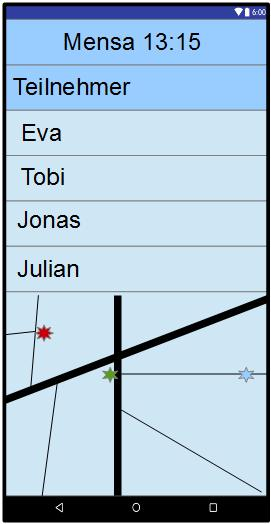
\includegraphics[width=.3\textwidth]{GUI_Termin.jpg}
	\newline
	Von dieser Activity kann ein Benutzer zu folgenden Activities navigieren:
	\begin{itemize} 
	 \item GroupActivity 
	 \end{itemize}
	 
	\subsubsection {NewEventActivity}
	Die NewEventActivity lässt einen Benutzer ein neues Event erstellen.
	\newline
	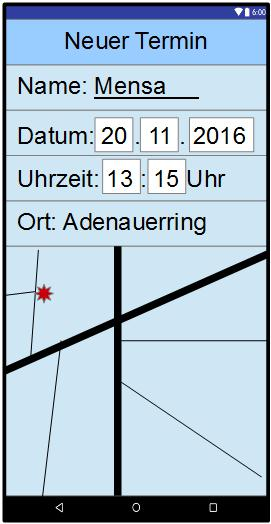
\includegraphics[width=0.3\textwidth]{GUI_NeuerTermin.jpg}
	\newline
	Services die von dieser Activity gestartet werden:
	\begin{itemize}
	\item EventService
	\end{itemize}
	Von dieser Activity kann ein Benutzer zu folgenden Activities navigieren:
	\begin{itemize} 
	 \item GroupActivity
	 \end{itemize}
	 
	 \subsubsection{Fragments}
	 Fragments sind Teile einer Activity, welche unabhängig voneinander und vom Layout geladen und mit Funktionalität bestückt werden können.  
	 Sie können nur innerhalb von Activities existieren, sind aber leicht austauschbar und ein Fragment kann auch in mehreren Activities eingesetzt werden. 
	 Sie bilden somit die Grundlage für ein dynamisches Layout. \newline
	 Unser Ziel ist es, Activities in agile Fragments zu unterteilen, um ein möglichst anpassungsfähiges Layout zu erhalten, welches sich auch leichter auf weitere Geräte, wie zum Beispiel Tablets übertragen lässt.
	 \newline Einige Fragments welche wir einsetzen werden:
	 \begin{itemize}
	 \item Maps Fragment: Ein Fragment, in dem den Nutzern die Karte mit allen Standorten bereitgestellt wird. Wird in der NewEventActivity und der EventActivity benötigt.
	 \item FounderFragment: In der GroupInfoActivity werden dem Gründer der Gruppe mehr Informationen als einem normalen Mitglied bereitgestellt. Dies ermöglichen wir in dem dieses spezifische Fragment in die selbe Activity geladen wird.
	 \item MemberFragment: Das Gegenstück zum FounderFragment. Wird für ein normales Mitglied in die GroupInfoActivity geladen.
	 \end{itemize}
	 
	
	\subsection{edu.kit.pse.gruppe1.goApp.client.model}
	Das Modell entspricht \hyperlink{ServerModel}{dem Modell des Servers} ist aber natürlich auch auf dem Clienten zu implementieren, eine zusätzliche Beschreibung ist an dieser Stelle aber nicht nötig.
	
	\subsection{edu.kit.pse.gruppe1.goApp.client.controler.serverConnection}
	Das Package serverConnection wird vom Clienten benötigt um die Anfragen der Services weiterzuleiten und so eine Kommunikation zum Server herzustellen. Es ist demnach auf dem Clienten implementiert. Eine Beschreibung der Klassen findet sich aber \hyperlink{ServerConnection}{hier}, da sie thematisch besser in das Kapitel Kommunikation Server \& Client passt.